%# -*- coding: utf-8-unix -*-
%%==================================================
%% chapter02.tex for SJTU Master Thesis
%%==================================================

\chapter{Shuffle特点观察}
\label{chap:observations}

本章首先分析了shuffle在目前分布式DAG计算框架中的特性,然后通过对其特征的研究,结合分布式DAG计算框架的特性,探索其优化的方向。

\section{Shuffle的特点}
在分布式并行DAG计算框架中,shuffle被用来实现一个在计算过程中任务的多对多数据依赖。
同时也代表了一次计算集群内部节点多对多的网络数据传输。
为了便于理解,本文用map阶段来代表产生shuffle数据的DAG计算阶段,用reduce阶段代表获取shuffle数据作为输入的计算阶段。

在图\ref{fig:workflow}中,我们呈现了一个shuffle在现有框架中的中局部的具体计算流程, 该流程由两个map任务和一个reduce任务组成。
如图\ref{fig:workflow}所示,其中的shuffle write表示一个map任务将计算产生的中间结果写入到本地磁盘的过程。
这个过程会在map任务完成对所有输入数据的计算之后开始。
在每一个map任务内部,计算框架会根据用户定义的计算方法和现阶段的数据,对于其中一个数据分区(partition)进行计算。
计算完成之后,map任务就会根据用户定义的分区函数(比如哈希分区或者排序分区),将计算产生的中间结果(键值对)进行分块存储。
其中存储这些代表中间结果的键值对的数据块的数目等同于下一个计算阶段(reduce)的任务数目。
这些分块的数据即在shuffle阶段通过网络传输的数据。这些数据块往往会在分块结束之后被写入本地磁盘。

在reduce阶段开始真正的计算之前,首先要通过网络从远程的节点的磁盘上拉取map阶段产生的属于该任务输入的部分shuffle数据块,即图\ref{fig:workflow}中的shuffle read部分。

可以看到在传统的DAG计算框架中,受限于粗粒度的资源调度机制,无论是shuffle write还是shuffle read都是由计算任务(task)来执行这部分I/O密集型的操作。
正因为这种粗粒度的调度和集成在计算任务中的I/O操作,使得硬件资源的复用性严重受损,进而损害了计算框架本身的性能。
有相关研究表明,Yahoo!公司中60\%的MapReduce工作和Facebook公司中20\%的MapReduce工作中存在大量的shuffle数据\cite{shufflewatcher}。
对于这些存在大量shuffle的工作中,shuffle传输所带来的延迟甚至会成为整个工作完成时间的瓶颈。
比如在一份Facebook公司公开的MapReduce任务日志中,shuffle过程的平均占用了整个工作完成时间的33\%。
对于那些存在大量shuffle的工作,shuffle的开销甚至最多占用了整个工作完成时间的70\%。

\begin{figure}[!htp]
	\centering
	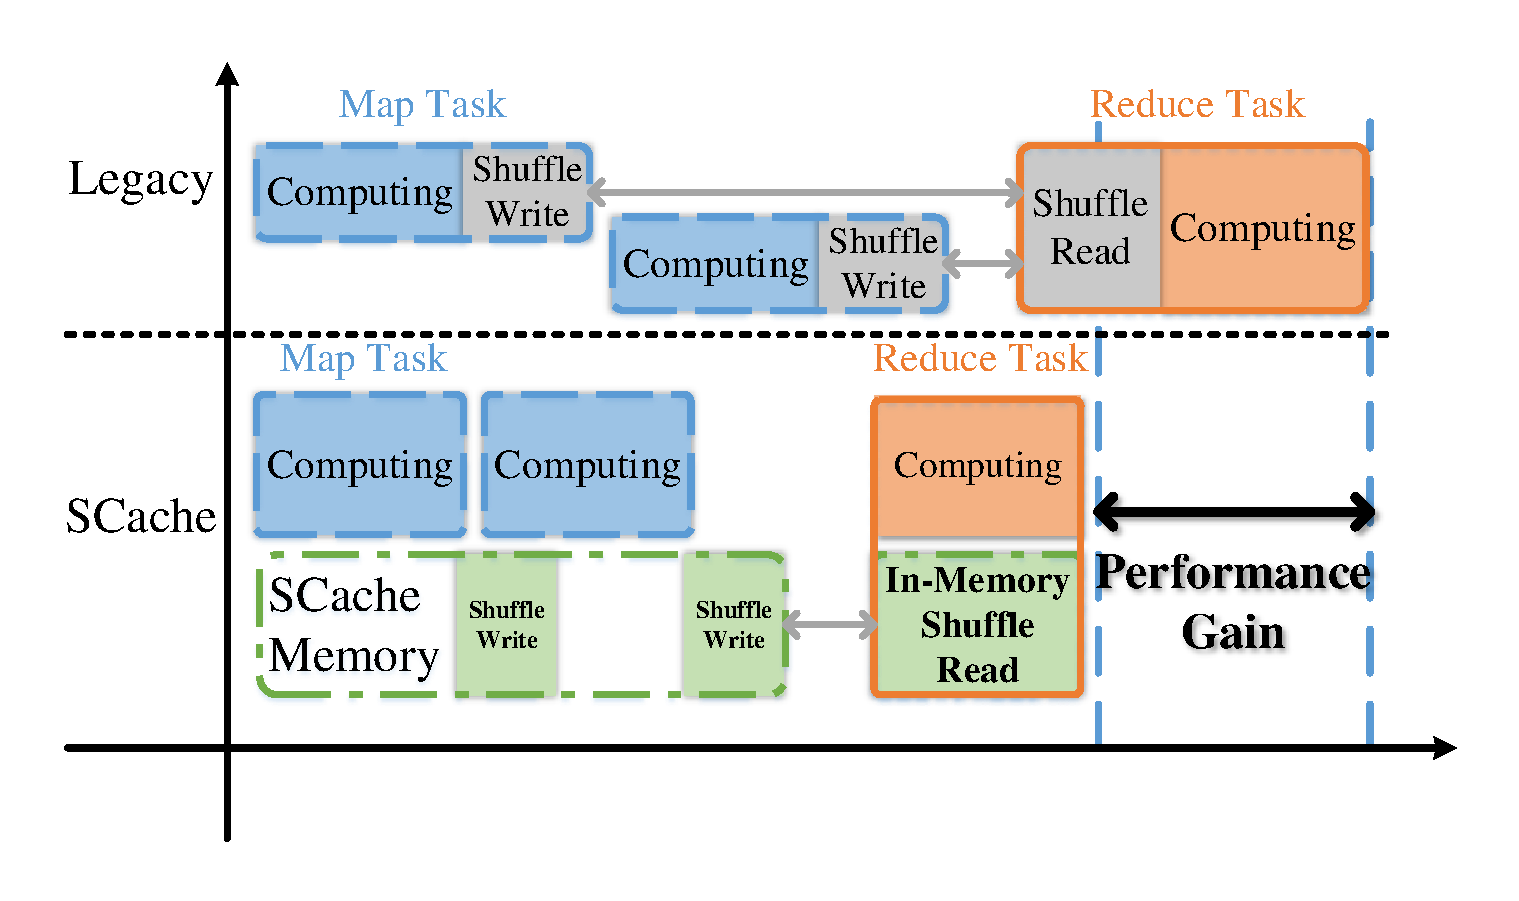
\includegraphics[width=\textwidth]{../../PPoPP-2018/fig/workflow.pdf}
	\bicaption[fig:workflow]{传统分布式DAG计算框架工作流程与在SCache协同下工作流程的比较}{传统分布式DAG计算框架工作流程与在SCache协同下工作流程的比较}{Fig}{Workflow Comparison between Legacy DAG Computing
	Frameworks and Frameworks with SCache}
\end{figure}

\section{对shuffle的观察}

为了满足计算逻辑中的部分依赖,shuffle这个过程在分布式DAG的计算过程中是无法避免的。
但是我们能不能通过改进shuffle的过程来减少其对计算框架性能的影响呢?
为了探索对其优化的可能性,我们在一个由5个Amazon AWS EC2 m4.xlarge\cite{aws}节点组成的集群中运行了一些具有代表性的Spark应用。
在运行这些应用的同时,我们测量了每个节点的CPU利用率,磁盘和网络的吞吐率,并且收集了每个应用的执行信息。
在图\ref{fig:util}中,我们展示了在运行一个Spark GroupByTest应用时一个节点上的硬件资源利用率随时间变化的结果。
Spark GroupByTest是一个包含两轮计算阶段,中间通过一次shuffle连接的简单应用。
图中的“execution”部分表示了从第一个计算任务启动到最后一个计算任务结束的时间,
“shuffle write”阶段表示从第一个任务shuffle数据块被写入开始到最后一个任务的最后一个数据块写入结束的时间,
“shuffle read and execution”则表示从第一个reduce任务开始获取shuffle数据并执行到所有reduce任务执行结束的时间。

从单节点的硬件资源率用率和任务执行的时间分布,结合多个节点的这部分数据,我们发现以下一些问题。

\begin{figure}[!htp]
	\centering
	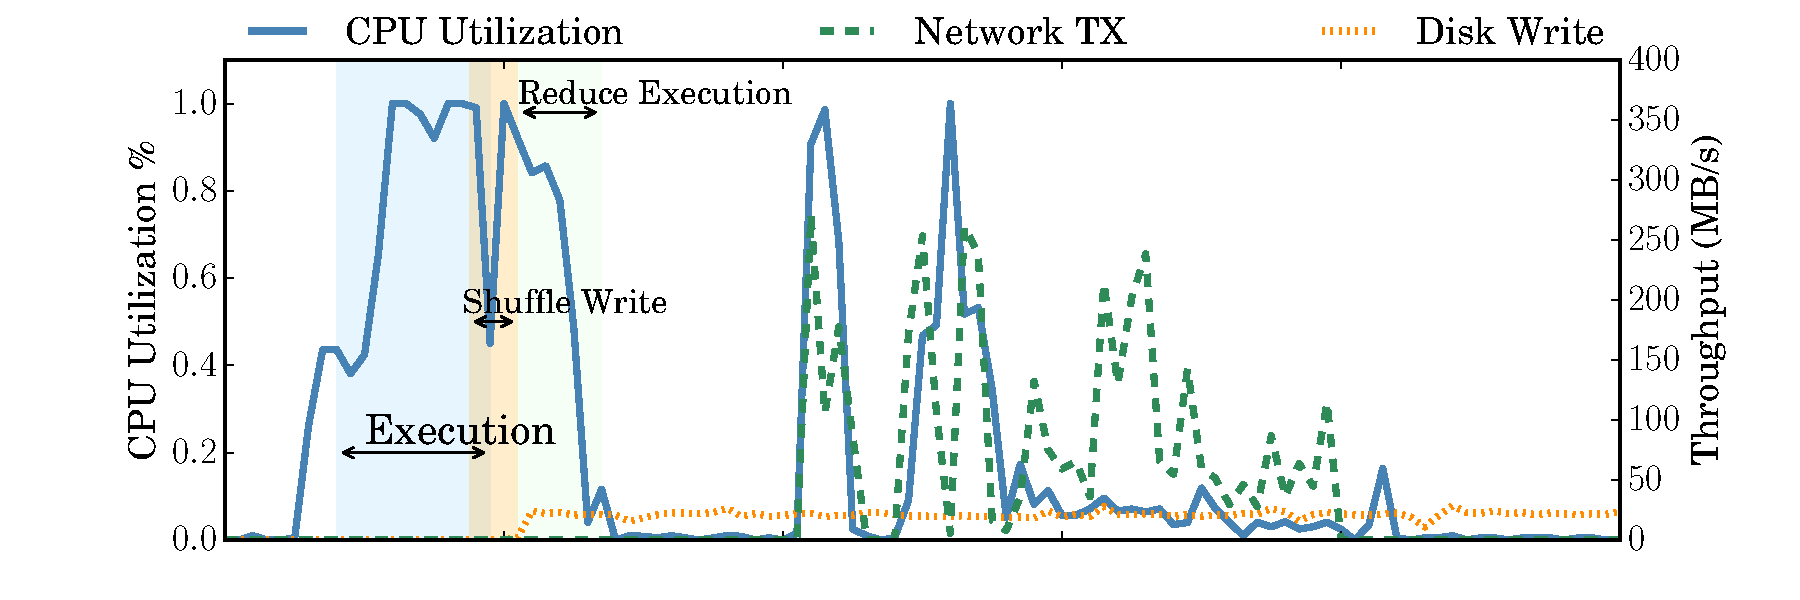
\includegraphics[width=\textwidth]{../../PPoPP-2018/fig/util.pdf}
	\bicaption[fig:util]{运行包含一个shuffle的Spark应用时的硬件资源利用率}{运行包含一个shuffle的Spark应用时的硬件资源利用率}{Fig}{CPU utilization and I/O throughput of a node
	during a Spark single shuffle application}
\end{figure}

\subsection{粗粒度的资源分配}

在现有的硬件资源分配机制下,当一个slot被计算框架分配给一个任务的时候,只有在该任务执行结束,这个slot以及其对应的硬件资源才会被释放。
对于一个map任务的技术是在他完成了shuffle write之后。
而在reduce任务一端,当一个reduce任务占用一个slot之后,它首先需要的只是通过一些I/O操作来获取shuffle数据。
而在图\ref{fig:util}中,可以看到shuffle数据的写入和shuffle数据的读取都是I/O密集型操作,在这两个阶段,slot中的CPU利用率很低。
反过来,在进行计算的过程中,节点上的I/O资源则被大量闲置。
由此可知,在目前DAG计算框架分配的任务的不同阶段对硬件资源的需求是不一致的。
但是当前这种主流的粗粒度资源分配方式为了满足任务在不同阶段的需求,只能舍弃一部分硬件资源的率用率。
因此要改变这种资源与需求的不匹配,必须提供一种更细粒度的资源分配机制。

\subsection{同步滞后的shuffle读取}

在目前的主流分布式DAG计算框架中,大多采用了Bulk Synchronous Parallel(BSP)模型来控制每个计算阶段。
因此当图\ref{fig:util}中的reduce阶段被调度时,集群中所有节点都会同时启动reduce任务。
而reduce任务启动之后首先需要通过网络来完成shuffle数据的读取。
结合图\ref{fig:util}可以发现,在“shuffle read”阶段,该节点的网络产生了一个瞬时的流量高峰,而此时集群中其他节点也会产生相应的流量高峰。
这种几乎同时的流量高峰的出现,会对整个集群的网络带来巨大的压力,极易造成链路上的拥塞。
而当网络检测到拥塞时,无论是传统的TCP\cite{tcp}还是更先进的DCTCP\cite{dctcp}都会降低传输速率。
同时拥塞的发生还可能导致网络中交换机的丢包和重传。
这些因素都会减慢shuffle读取的速率,延长了shuffle读取过程,进而损害了reduce阶段的性能。

\subsection{低效率的磁盘操作}
\label{subsec:size}

在整个shuffle过程中,至少存在两次磁盘操作,即map阶段的shuffle数据写入磁盘和reduce阶段从远程磁盘读取shuffle数据。
在前文中提到的粗粒度的资源分配机制是的计算任务中的I/O操作都会阻塞CPU内存等计算资源的释放和利用。
而其中大量的磁盘操作更加剧了这个阻塞带来的延迟。

为了解决阻塞带来的延迟,首先需要回答两个问题:shuffle数据在磁盘的持久化是否必要;如果持久化是必要的,那么能否通过异步的方式来隐藏磁盘操作的开销。
对于必要性,在当下数据中心内存日益增大的背景下,为了节约内存而采用的将shuffle数据写入磁盘的方式(spill)并没有那么强的必要性。
而且相较于应用的输入数据而言,shuffle数据作为中间结果,其体积要相对小很多。
比如Spark Terasort\cite{spark-tera}中,shuffle数据只占到了输入数据的25\%不到。
在一些研究中\cite{makingsense}的数据也表明,shuffle数据大约只占到了输入数据的10\% $\sim$ 20\%。
从另一个角度来看,目前出现了越来越多的基于内存的分布式存储系统,比如memcached\cite{memcached},Tachyon\cite{tachyon}(现在的Alluxio\cite{alluxio})以及RAMCloud\cite{ramcloud}等。
这个趋势间接表面了在目前的数据中心环境下,内存资源是足够用来存放这些数据的。
同时,由于DAG的存在,结合调度算法可以很容易就获取任务的调度顺序。
在这个前提下,即使内存资源十分紧张,shuffle的数据也可以通过异步预取的方式,提前从磁盘获取。
因此我们任务,目前在shuffle过程中低效率的磁盘操作是可以被优化的。

\subsection{多轮任务执行}

在运行分布式DAG计算工作的时候,对于每一阶段的计算任务,无论是经验还是这些框架的手册都推荐在开发应用时将每个计算阶段并行的任务划分成多轮。
即对于一个有$s$个计算slot的计算集群而言,每个计算阶段的并行任务$t$:
\begin{equation}
	\label{eq:multi}
	t = k \times x \quad (k = 1, 2, 3, ...)
\end{equation}
比如Hadoop MapReduce的手册\cite{hadooptutorial}建议每个节点运行10-100个map任务(即等式\ref{eq:multi}中 $k \in [10, 100]$)。
同时该手册还建议运行时任务时将任务的并发度调整到$0.95$ 或 $1.75 \times$ 节点数 $\times$ 每个节点的最大容器数。
Spark的配置手册\cite{sparkconf}也建议为节点上的每个CPU分配2-3个任务(即等式\ref{eq:multi}中 $k = 2, 3$)。

对于shuffle数据而言,当每一个map任务运行结束时,该任务所产生的shuffle数据就能被完整的获取。
于此同时,结合图\ref{fig:util},可以观察到在任务执行过程中,网络一直处于闲置状态。
因此在多轮任务执行的应用环境当中,如果shuffle传输的目的节点已知,那么shuffle数据便可以在map阶段的执行过程中进行预取。
这种多轮任务的属性则可以很好的将shuffle数据传输过程进行重叠。

\section{本章小结}
通过以上的观察和分析,我们认为shuffle存在继续优化的空间。
具体来讲,就是通过解耦合的方式移除阻塞式的I/O操作,然后利用多轮任务执行的特性对shuffle数据进行预取,同时通过内存数据缓存来进一步加速shuffle的读写。
基于上述优化目标,我们提出了SCache针对分布式DAG计算框架shuffle过程的优化系统。
在图\ref{fig:workflow}的下半部分展现了DAG计算框架与SCache协同工作时的工作流程。
在shuffle write阶段,SCache通过内存拷贝的方式讲数据直接从任务的内存空间拷贝到预留的shuffle数据存储内存区域。
于此同时,磁盘的写操作将被省略。而由框架分配的slot资源也会在内存拷贝结束之后被立即释放。
这些缓存在内存中的shuffle数据会在SCache完成对reduce任务的预调度之后立刻进行网络传输。
这种预传输方式既能将shuffle read阶段的时间很好的隐藏在map任务执行的过程中,又能避免传统DAG计算框架统一调度带来的同步瞬时大量的网络吞吐。

为了实现以上优化:
\begin{itemize}
	\item Shuffle的过程必须从计算任务中解耦,从而实现更细粒度的资源分配和更高的资源利用率。
	\item Reduce任务必须在map阶段就进行预调度,从而实现shuffle数据预取。同时在预调度的过程中不能真正启动reduce任务,以防其占用计算资源。
	\item 需要结合DAG计算逻辑实现精细化shuffle数据内存缓存管理,进一步加快shuffle读写速度。
	\item 为了实现跨框架的优化方案,shuffle过程必须被独立到计算框架外部进行管理,并且实现一个具有通用性的API。
\end{itemize}
